\thispagestyle{toancuabinone}
\pagestyle{toancuabi}
\everymath{\color{toancuabi}}
%\blfootnote{$^1$\color{toancuabi}Đại học Thăng Long.}
\graphicspath{{../toancuabi/pic/}}
\begingroup
\AddToShipoutPicture*{\put(0,616){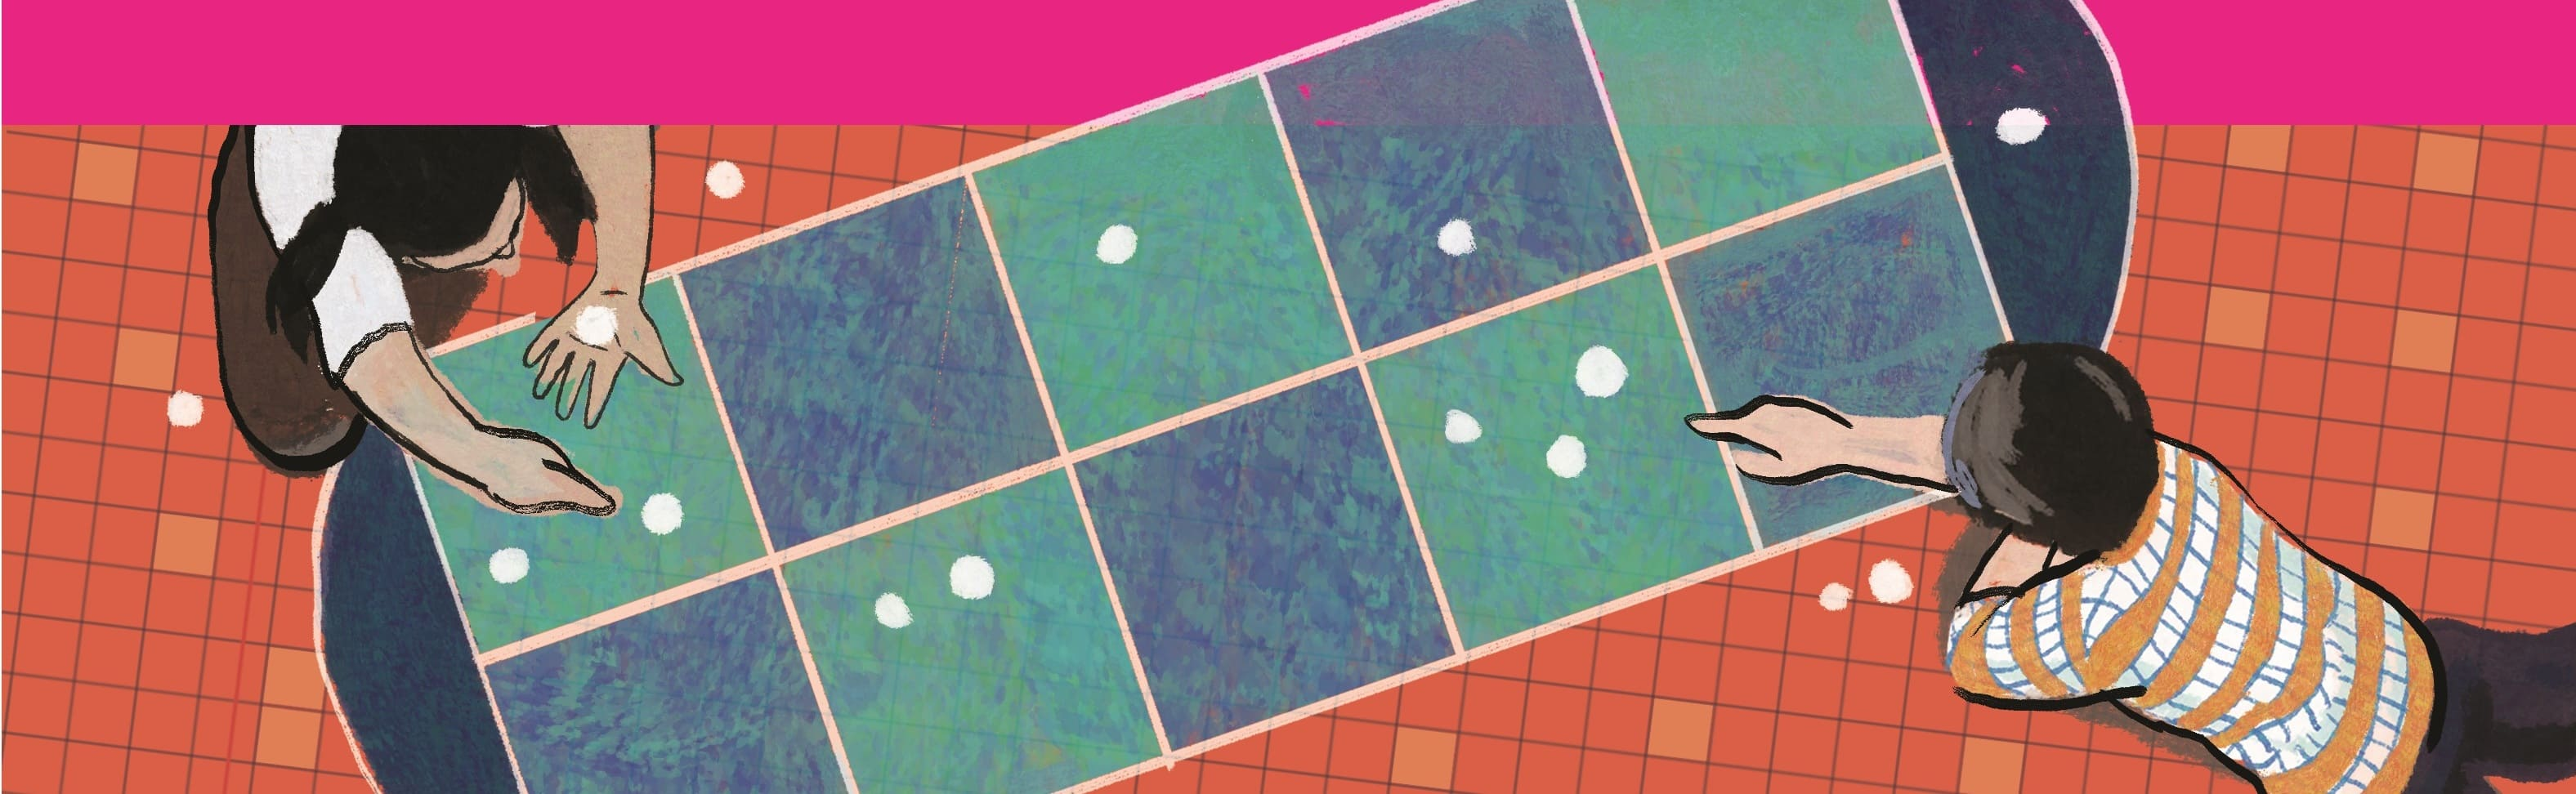
\includegraphics[width=19.3cm]{../bannertoancuabi}}}  
\AddToShipoutPicture*{\put(78,550){
\includegraphics[scale=1]{../tieude.pdf}}} 
\centering
\endgroup
\vspace*{160pt}

\begin{multicols}{2}
	Thám tử Xuân Phong cùng thanh tra Lê Kính tham gia một buổi giới thiệu sản phẩm của hai công ty là Tae Yeon và TeaYon tại triển lãm Điện tử Expo -- New Vision của khu vực. Công ty  Tae Yeon có uy tín từ lâu đời, với những sản phẩm tinh tế có chất lượng tốt nổi tiếng,  các nhân viên của công ty luôn nói thật. Còn công ty TeaYon chuyên sản xuất đồ rẻ, kém chất lượng, bắt chước kiểu dáng của công ty Tae Yeon nên ban giám đốc dặn các nhân viên của mình chỉ được nói dối trong buổi triển lãm. 
	\vskip 0.1cm
	Vừa đặt chân tới khu vực triển lãm được trang hoàng lộng lẫy, Xuân Phong gặp ngay $5$ đại diện  của hai công ty này đứng tại cổng ra vào và tươi cười niềm nở tiếp đón. Xuân Phong tiến tới họ và hỏi cả $5$ người cùng một câu hỏi ``Có bao nhiêu người đến từ công ty Tae Yeon trong số các bạn?" 
	\vskip 0.1cm
	Người thứ nhất trả lời ``Không có ai cả". Hai người tiếp theo đều trả lời ``Có đúng một người". 
	\vskip 0.1cm
	Vậy hai người còn lại sẽ trả lời câu hỏi của thám tử Xuân Phong như thế nào nhỉ? Em có thể suy đoán ra câu trả lời của họ và giải thích lập luận được không?
%	
%	Người của công ty Tae Yeon không thể trả lời ``Không có ai cả" vì như vậy người đó sẽ nói dối. Vì vậy, người đầu tiên đến từ công ty TeaYon. 
%	\vskip 0.1cm
%	Hai người tiếp theo trả lời giống nhau, vì thế họ phải cùng nói thật hoặc cùng nói dối, tức là đến từ cùng một công ty.
%	\vskip 0.1cm
%	Nếu cả hai người này cùng đến từ công ty Tae Yeon, suy ra số người của công ty Tae Yeon trong số họ không ít hơn $2$ người. Suy ra câu trả lời của họ là sai. Vì vậy cả hai người thứ hai và thứ ba đều nói dối, tức là đến từ công ty TeaYon.
%	\vskip 0.1cm
%	Do vậy, trong số $5$ người này, có ít nhất $3$ người của công ty TeaYon và không quá $2$ người đến từ công ty Tae Yeon.
%	\vskip 0.1cm
%	Nhưng vì cả $3$ người đầu tiên đều nói dối, suy ra số người của công ty Tae Yeon trong số họ không thể là $0$ hoặc $1$. Vì vậy, cả hai người còn lại đều là nhân viên của công ty Tae Yeon. Và họ đều sẽ trả lời là ``Có hai người".
\end{multicols}
	\begin{figure}[H]
		\centering
		\vspace*{-5pt}
		\captionsetup{labelformat= empty, justification=centering}
		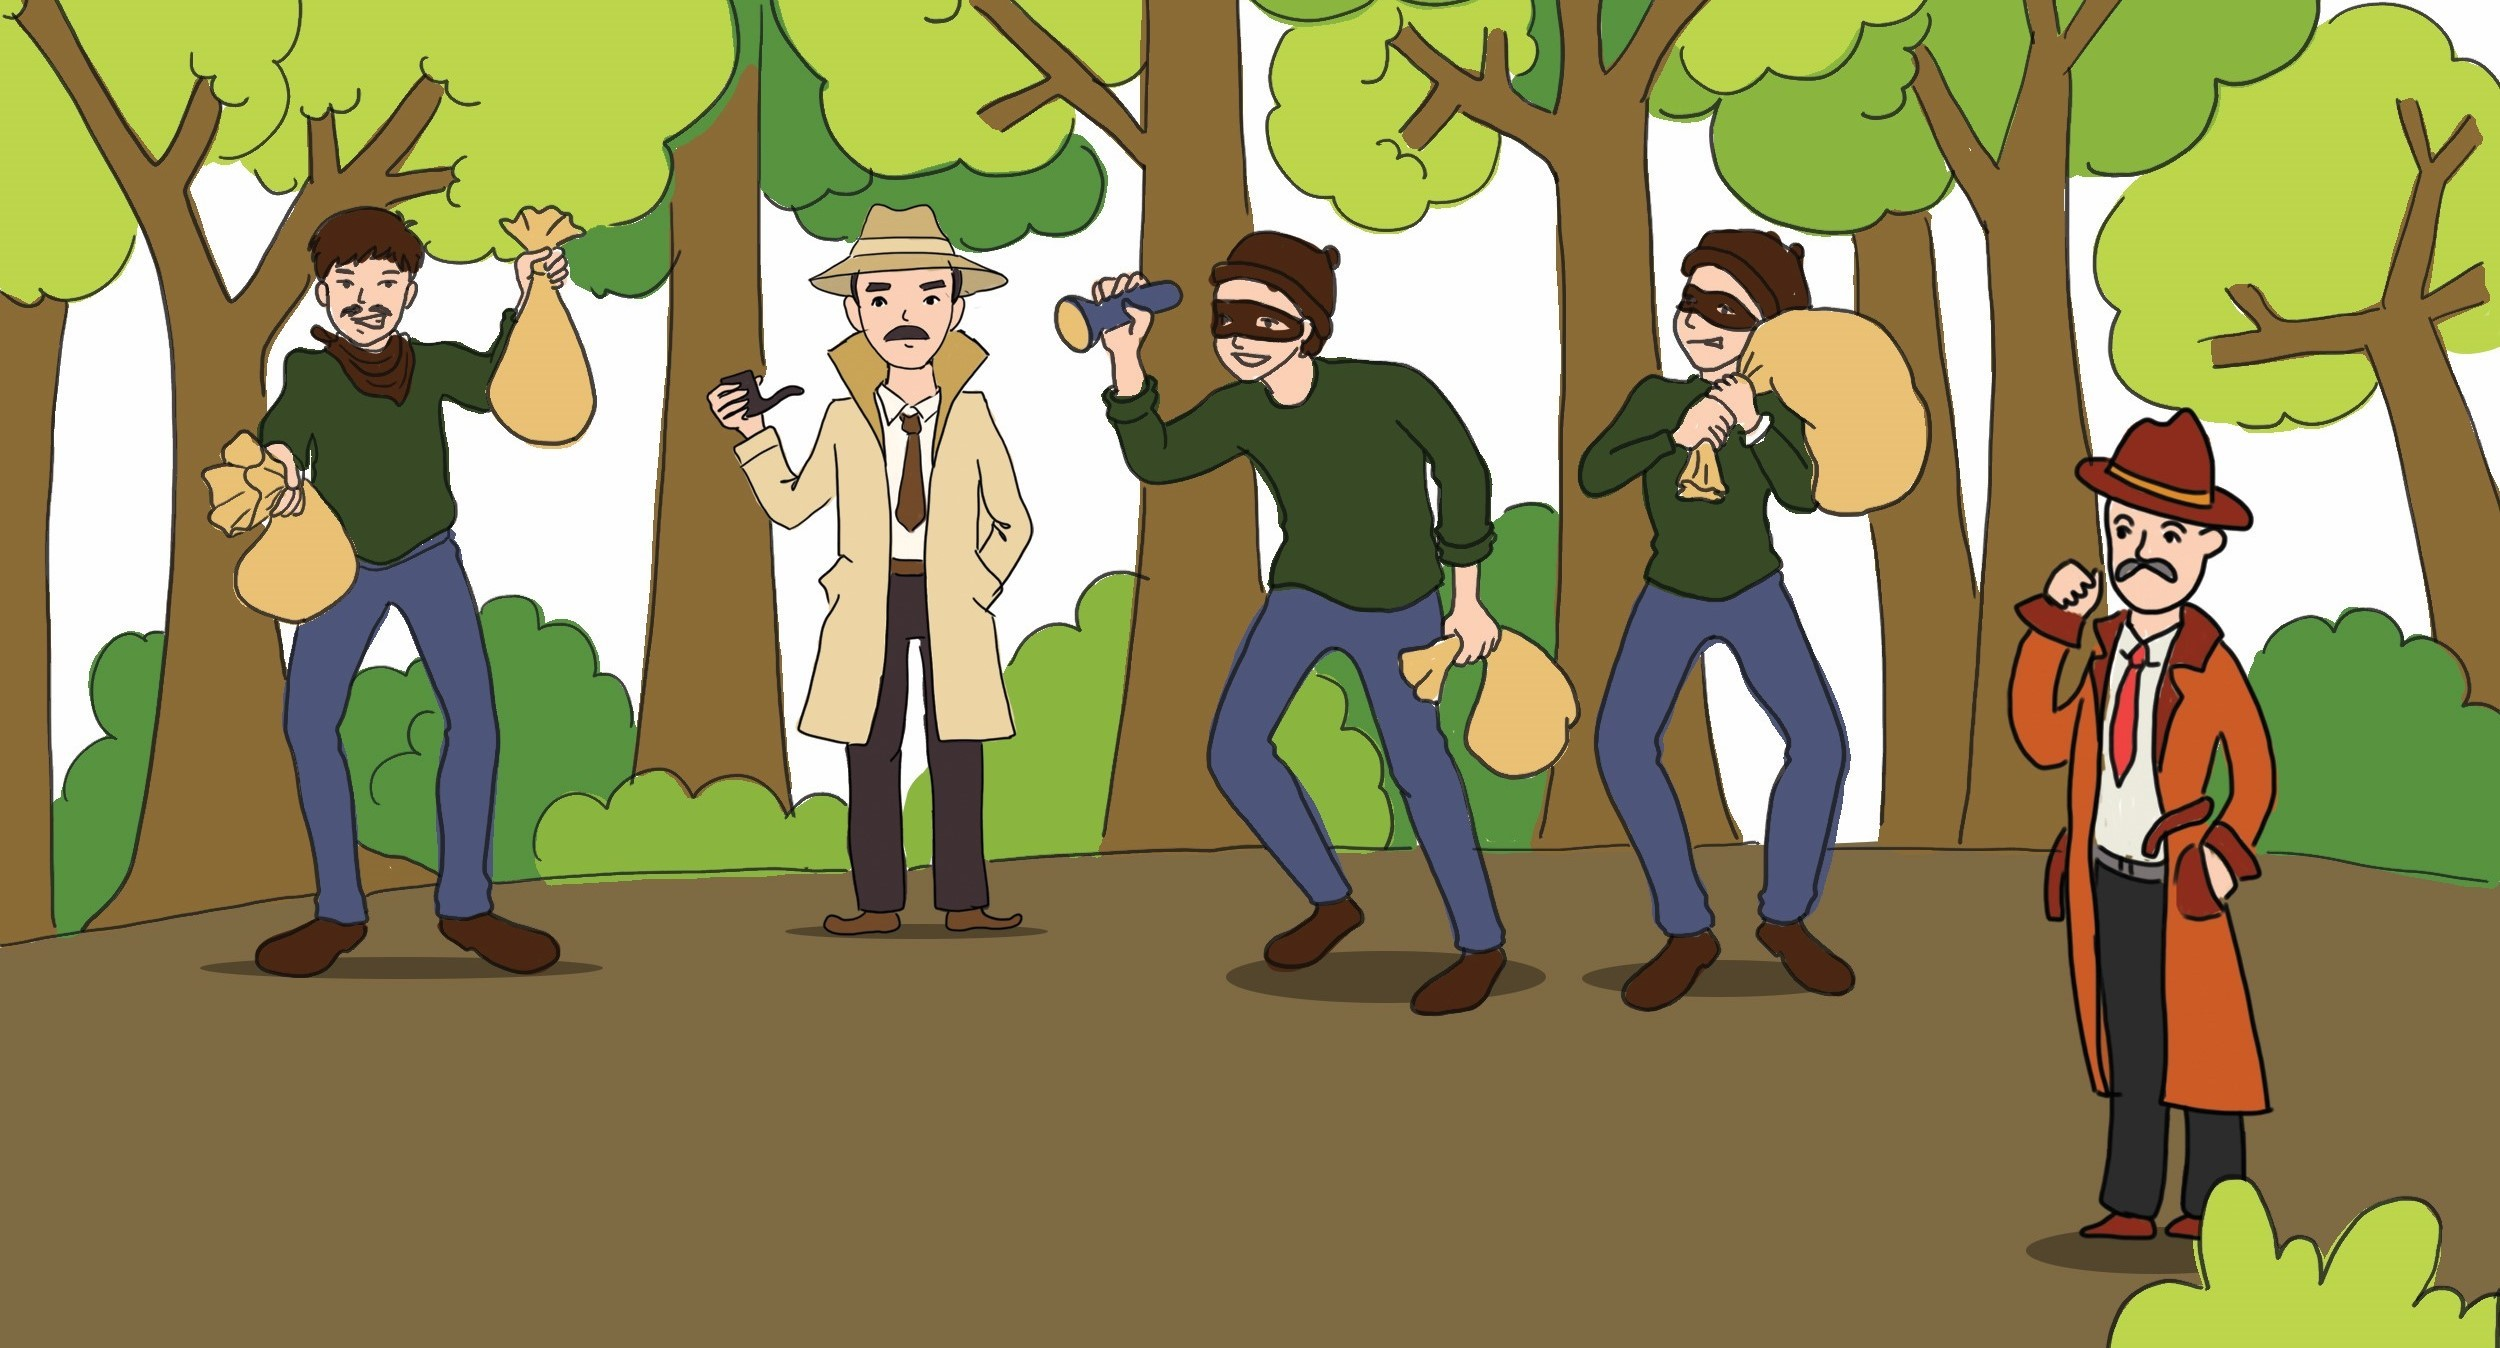
\includegraphics[width=1\linewidth]{xuanphong}
		\vspace*{-5pt}
		\end{figure}
\newpage
\begingroup
\AddToShipoutPicture*{\put(115,670){
\includegraphics[scale=1]{../tieude11.pdf}}} 
\centering
\endgroup
\vspace*{33pt}

\begin{multicols}{2}
	$\pmb{1.}$	Trong một cuộc thi thể thao, ban tổ chức chọn ra một số bạn học sinh ở lớp $5A$ và một số bạn ở lớp $5B$ thi đấu trực tiếp. Mỗi bạn ở lớp $5A$ được chọn ra sẽ thi đấu duy nhất một trận với một bạn ở lớp $5B$, và ngược lại, mỗi bạn ở lớp $5B$ được chọn ra chỉ đấu đúng một trận với một bạn ở lớp $5A$. Biết rằng số học sinh lớp $5A$ được chọn thi đấu chiếm $2/3$ tổng số học sinh toàn lớp $5A$, còn số học sinh lớp $5B$ được chọn thi đấu chiếm $3/5$ tổng số học sinh toàn lớp $5B$. Tổng số học sinh của cả hai lớp là $57$ bạn. Hỏi có bao nhiêu học sinh của hai lớp đã tham gia các trận thi đấu trực tiếp?
	\begin{figure}[H]
			\centering
			\vspace*{-5pt}
			\captionsetup{labelformat= empty, justification=centering}
			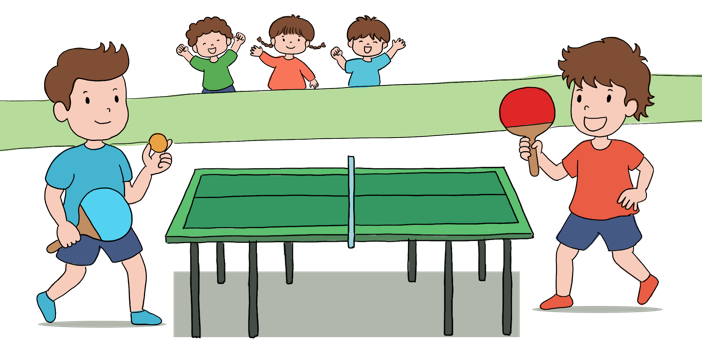
\includegraphics[width=1\linewidth]{Pi5_bai1}
			\vspace*{-15pt}
		\end{figure}
	$\pmb{2.}$ Công ty vận tải được thông báo ngắn gọn là có một số kiện hàng có tổng trọng lượng là $10$ tấn cần được vận chuyển, hơn nữa mỗi kiện hàng nặng không quá $1$ tấn. Hỏi công ty  cần điều động ít nhất bao nhiêu xe tải có trọng tải là $3$ tấn mỗi xe để luôn chắc chắn chở được hết được số hàng hoá đó?
	\begin{figure}[H]
			\centering
			\vspace*{-10pt}
			\captionsetup{labelformat= empty, justification=centering}
			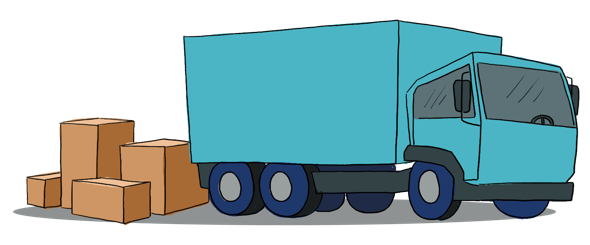
\includegraphics[width=1\linewidth]{Pi5_bai2}
			\vspace*{-15pt}
		\end{figure}
	$\pmb{3.}$ Sau khi được sạc đầy pin, điện thoại di động của bạn An dùng đúng $6$ tiếng ở chế độ trò chuyện hoặc đúng $210$ tiếng ở chế độ chờ. Khi bạn An lên tàu hoả để đi du lịch, pin của bạn được sạc đầy $100\%$, và trên tàu không có ổ cắm sạc nên khi xuống ga, pin của bạn cũng vừa hết sạch. Biết rằng An đã nói chuyện với bạn bè đúng một nửa thời gian khi ngồi trên tàu, còn nửa thời gian còn lại đặt điện thoại ở chế độ chờ. Hỏi thời gian An đi trên tàu hoả là bao nhiêu lâu?
	\begin{figure}[H]
			\centering
			\vspace*{-5pt}
			\captionsetup{labelformat= empty, justification=centering}
			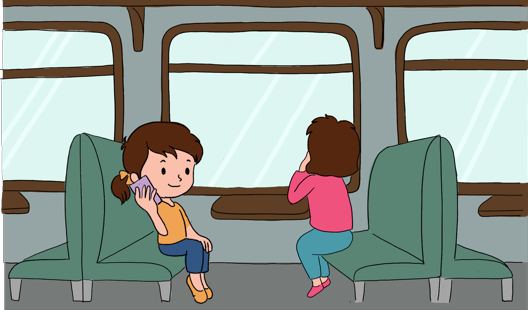
\includegraphics[width=1\linewidth]{Pi5_bai3}
			\vspace*{-15pt}
		\end{figure}
	$\pmb{4.}$ Một nhóm học sinh đi bộ từ điểm hẹn tới bến xe buýt để kịp đón chuyến xe vào lúc $8$ giờ. Cũng vào thời điểm này, từ điểm thăm quan, một chiếc xe buýt cũng xuất phát để tới kịp bến xe đón nhóm học sinh đó. Tuy  nhiên nhóm học sinh tới bến xe buýt khá sớm, vào lúc $6$ giờ $10$ phút, nên họ quyết định đi bộ tiếp tới điểm thăm quan. Trên đường, các bạn đã gặp được xe buýt và lên xe đi tiếp.  Cuối cùng cả nhóm đến được điểm thăm quan sớm hơn $20$ phút so với thời gian ấn định. Biết rằng vận tốc của xe buýt là $60$ km/h và vận tốc đi bộ của các em học sinh luôn không đổi. Hãy tìm vận tốc đi bộ của nhóm học sinh trước khi gặp xe buýt.
	\begin{figure}[H]
			\centering
			\vspace*{-5pt}
			\captionsetup{labelformat= empty, justification=centering}
			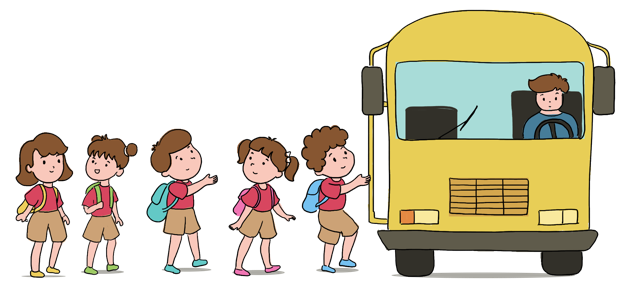
\includegraphics[width=1\linewidth]{Pi5_bai4}
			\vspace*{-10pt}
		\end{figure}
	$\pmb{5.}$ 	Có $100$ chiếc xe ô tô đỗ liền nhau thành một hàng dọc bên lề đường, trong đó có $70$ chiếc xe hiệu Mercedes, còn lại là những xe nhãn hiệu khác. Trong các xe nhãn hiệu Mercedes có $30$ chiếc màu đỏ, $20$ chiếc màu vàng và $20$ chiếc màu hồng. Biết rằng không có hai xe Mercedes nào khác màu lại đỗ cạnh nhau. Em hãy chỉ ra rằng luôn tìm ra $3$ chiếc xe Mercedes cùng màu đỗ liên tiếp nhau.
	\begin{figure}[H]
			\centering
			\vspace*{-5pt}
			\captionsetup{labelformat= empty, justification=centering}
			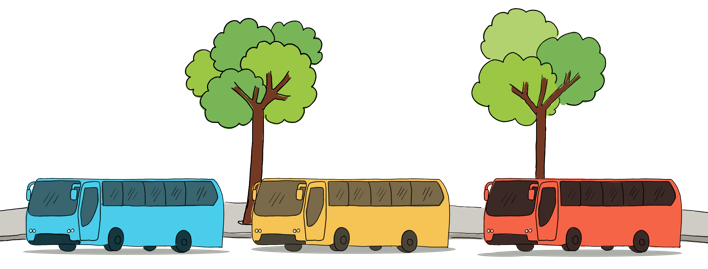
\includegraphics[width=1\linewidth]{Pi5_bai5}
			\vspace*{-15pt}
		\end{figure}
	$\pmb{6.}$ Một lớp học có $20$ em học sinh. Cô giáo chủ nhiệm của lớp tổ chức một số buổi thăm quan vào mỗi ngày cuối tuần trong suốt năm học, mỗi buổi tham quan có ít nhất $4$ em học sinh tham gia. Em hãy chứng minh rằng có một buổi thăm quan mà mỗi em học sinh tham gia buổi đó đều tham gia ít nhất $1/17$ tổng số tất cả các buổi tham quan của cả năm học.
	\begin{figure}[H]
		\centering
		\vspace*{-5pt}
		\captionsetup{labelformat= empty, justification=centering}
		
\includegraphics[width=1\linewidth]{Pi5_bai6}
		\vspace*{-15pt}
	\end{figure}
\end{multicols}
%\vspace*{-10pt}
%{\color{toancuabi}\rule{1\linewidth}{0.1pt}}
%\begingroup
%\AddToShipoutPicture*{\put(110,405){
\includegraphics[scale=1]{../tieude2.pdf}}} 
%\centering
%\endgroup
%\vspace*{75pt}
%
%\begin{multicols}{2}
%	$\pmb{1.}$ Hai anh bạn rủ nhau đi câu cá. Khi được hỏi ``Trong mỗi giỏ của các anh có bao nhiêu con cá đấy?" thì anh thứ nhất trả lời ``Trong giỏ của tôi có số cá bằng nửa số cá ở giỏ của anh kia và thêm $10$ con nữa". Anh thứ hai lại nói ``Còn trong giỏ của tôi có số cá bằng số cá trong giỏ của anh kia và thêm $20$ con nữa". Vậy cả hai anh bạn có tất cả bao nhiêu con cá nhỉ? 
%	\begin{figure}[H]
	%		\centering
	%		\vspace*{-10pt}
	%		\captionsetup{labelformat= empty, justification=centering}
	%		\includegraphics[width=1\linewidth]{Pi10_ToanBi_Bai1}
	%		\vspace*{-15pt}
	%	\end{figure}
%	\textit{Lời giải.} Một nửa số cá của anh thứ hai sẽ là nửa số cá của anh thứ nhất cộng thêm $10$ con. Vậy nửa số cá của anh thứ hai cộng thêm $10$ con sẽ bằng nửa số cá của anh thứ nhất cộng thêm $20$ con. Theo đề bài, số cá này bằng cả số cá của anh thứ nhất.
%	\vskip 0.1cm
%	Vậy một nửa số cá của anh thứ nhất là: $20$ (con)
%	\vskip 0.1cm
%	Suy ra anh thứ nhất có số cá là
%	\begin{align*}
	%		2 \times 20 = 40 \text{  (con)}
	%	\end{align*}
%	và anh thứ hai có số cá là 
%	\begin{align*}
	%		40+20 = 60 \text{  (con).}
	%	\end{align*} 
%	Tổng số cá của cả hai anh là 
%	\begin{align*}
	%		40+60 = 100 \text{  (con).}
	%	\end{align*}
%	Đây là bài tập đơn giản, tuy nhiên các em thử tập làm bằng nhiều cách khác nhau thông qua suy luận thông thường mà không cần dùng tới cách lập phương trình nhé.
%	\vskip 0.1cm
%	$\pmb{2.}$ Lọ lem có $100$ rổ đựng hạt dẻ, lúc đầu số hạt dẻ trong mỗi rổ là như nhau. Lọ Lem lấy đi trong rổ thứ nhất một số hạt dẻ, lấy từ rổ  thứ hai một số hạt gấp đôi như thế, lấy từ rổ thứ ba một số hạt gấp ba như thế, và cứ như vậy. Cuối cùng thì trong rổ thứ $100$ chỉ còn đúng một hạt dẻ, và còn lại ở tất cả trong $100$ rổ tổng cộng là $14950$ hạt dẻ. Hỏi ban đầu trong mỗi rổ có bao nhiêu hạt dẻ?
%	\begin{figure}[H]
	%		\centering
	%		\vspace*{-10pt}
	%		\captionsetup{labelformat= empty, justification=centering}
	%		\includegraphics[width=1\linewidth]{Pi10_ToanBi_Bai2}
	%		\vspace*{-15pt}
	%	\end{figure}
%	\textit{Lời giải.} 	Gọi số hạt dẻ mà Lọ Lem lấy ở rổ thứ nhất là $a$, khi đó tổng cộng số hạt dẻ mà Lọ lem đã lấy đi ở $100$ rổ là
%	\begin{align*}
	%		a+ 2a+\cdots+100a=5050a.
	%	\end{align*} 
%	Do rổ cuối cùng còn lại $1$ hạt dẻ nên ban đầu số hạt dẻ ở rổ cuối cùng (cũng là số hạt dẻ ở các rổ khác) là: $100a+1$ (hạt).
%	\vskip 0.1cm
%	Vậy, ban đầu tổng số hạt dẻ là
%	\begin{align*}
	%		100\times(100a+1) = 10000a+100 \text{  (hạt).}
	%	\end{align*} 
%	Ta có hệ thức là: $10000a+100-5050 a =14950$. Từ đó suy ra $a=3$. Vì vậy ban đầu mỗi rổ có  $100\times 3+1 = 301$ hạt dẻ.
%	\vskip 0.1cm
%	$\pmb{3.}$ Hai bạn học sinh là Nam và Vũ gặp nhau tại nhà của Vũ. Nam nói ``Nếu lấy số nhà của tớ là một số có hai chữ số trừ đi số có hai chữ số tạo thành khi viết theo thứ tự ngược lại, thì sẽ ra số nhà của cậu. Vậy tớ sống ở số nhà nào?"
%	\vskip 0.1cm
%	Vũ trả lời ``Ôi, bài toán này dễ quá" -- và giải ra luôn đáp số.
%	\vskip 0.1cm
%	Vậy các bạn đó sống ở những số nhà nào nhỉ?
%	\vskip 0.1cm
%	\textit{Lời giải.} 	Nếu thực hiện phép trừ của Nam, ta sẽ nhận được số có dạng $9\times k$, ở đó $k$ là hiệu của chữ số hàng chục và chữ số hàng đơn vị. Vì số viết theo thứ tự ngược lại cũng là số có hai chữ số, nên $k\le8$. 
%	\vskip 0.1cm
%	Nếu $k<8$ thì có thể thấy có nhiều số có hai chữ số (là số nhà) mà sau khi làm phép tính trừ đã cho sẽ cho kết quả như nhau. Khi đó Vũ không thể giải được ngay câu đố của Nam. Do đó $k=8$. Các em có thể tìm thấy số nhà của Nam là $91$, và số nhà của Vũ là $72$.
%	\begin{figure}[H]
	%		\centering
	%		\vspace*{-5pt}
	%		\captionsetup{labelformat= empty, justification=centering}
	%		\includegraphics[width=1\linewidth]{Pi10_ToanBi_Bai3}
	%		\vspace*{-15pt}
	%	\end{figure}
%	$\pmb{4.}$ Lớp của Hùng có $35$ học sinh. Trong số đó có $20$ em tham gia câu lạc bộ Toán, $11$ em tham gia câu lạc bộ Khéo tay, $10$ em không tham gia vào hai nhóm này. Hỏi có tất cả bao nhiêu em vừa tham gia CLB Toán lại vẫn không quên tham gia cả CLB Khéo tay nhỉ?
%	\begin{figure}[H]
	%		\centering
	%		\vspace*{-5pt}
	%		\captionsetup{labelformat= empty, justification=centering}
	%		\includegraphics[width=1\linewidth]{Pi10_ToanBi_Bai4}
	%		\vspace*{-15pt}
	%	\end{figure}
%	\textit{Lời giải.} 	Chúng ta chia toàn bộ số học sinh trong lớp thành bốn danh sách, mà không có em nào ở trong hai danh sách khác nhau, như sau. Danh sách ``toán thuần tuý" gồm các bạn chỉ tham gia CLB Toán, danh sách ``khéo tay thuần tuý" gồm các bạn chỉ tham gia CLB Khéo tay, danh sách ``giỏi toán lại khéo tay" gồm các bạn tham gia cả $2$ CLB  và cuối cùng là danh sách ``rảnh rỗi" là các bạn không tham gia vào hai CLB này. Theo đề bài, danh sách ``rảnh rỗi" có $10$ bạn, vì thế có $25$ bạn không ``rảnh rỗi". Trong số $25$ bạn này có $20$ bạn tham gia nhóm Toán, vì thế số ``khéo tay thuần tuý" là $5$ bạn. Vậy số bạn vừa tham gia nhóm Toán lại ``khéo tay" nữa là 
%	\begin{align*}
	%		11-5 = 6 \text{ (bạn).}
	%	\end{align*}
%	$\pmb{5.}$ Tùng đến trường mới có nhiều chuyện rất vui nên về khoe với bạn bè.
%	\begin{figure}[H]
	%		\centering
	%		%		\vspace*{5pt}
	%		\captionsetup{labelformat= empty, justification=centering}
	%		\includegraphics[width=1\linewidth]{Pi10_ToanBi_Bai5}
	%		\vspace*{-15pt}
	%	\end{figure}
%	-- Lớp tớ có $35$ học sinh. Và các cậu có tưởng tượng được không, mỗi người lại kết bạn với đúng $11$ học sinh cùng lớp.
%	\vskip 0.1cm
%	-- Không thể thế được! Bách, người bạn thân của Tùng vừa đạt giải trong một cuộc thi Olympic, ngay lập tức trả lời.
%	\vskip 0.1cm
%	Vì sao Bách lại nghĩ như vậy nhỉ?
%	\vskip 0.1cm
%	\textit{Lời giải.} 	Ta biểu diễn mỗi học sinh được thể hiện bởi một điểm. Nếu hai học sinh kết bạn với nhau ta sẽ nối hai điểm tương ứng bởi một đoạn thẳng. Như vậy có $35$ điểm, mỗi điểm được nối đúng với $11$ điểm khác. Khi đó tổng số các đầu của các đoạn thẳng nối quan hệ bạn bè là $35\times11$ là một số lẻ. Điều này là vô lý do mỗi đoạn thẳng thể hiện quan hệ bạn bè có đúng hai điểm đầu mút. 
%	\vskip 0.1cm
%	$\pmb{6.}$ Có $55$ em học sinh tham gia một cuộc thi Olympic. Tất cả các em đều nộp bài. Khi chấm bài, mỗi câu hỏi được chấm bởi một trong ba loại điểm: điểm ``$+$" nếu câu hỏi được trả lời hoàn toàn đúng; điểm ``$-$" nếu câu hỏi đã có trả lời nhưng chưa ra đúng đáp số; và điểm ``$0$" nếu câu hỏi chưa được trả lời. Sau khi chấm toàn bộ bài thi, ban tổ chức thấy không có hai bài thi nào có cả các số điểm ``$+$" và số điểm ``$-$" đồng thời trùng nhau. Vậy trong kỳ thi Olympic đó phải có ít nhất bao nhiêu câu hỏi?
%	\vskip 0.1cm
%	\textit{Lời giải.} 	Giả sử $a$ là số câu hỏi được ra.  Ta chia ra các trường hợp sau
%	\vskip 0.1cm
%	$1.$ Bài thi có tất cả các câu hỏi đều được trả lời: Khi đó số các bài thi sẽ không vượt quá $a+1$ bài: từ bài có $a$ dâú ``$+$" và $0$ dấu ``$-$" cho đến bài có $0$ dấu ``$+$" và $a$ dấu ``$-$".  
%	\vskip 0.1cm
%	Bài thi trong đó chỉ có đúng một bài chưa có trả lời (có một điểm ``$0$"): Số các bài thi  nhiều nhất là $a$ bài (từ $a-1$ điểm ``$+$" và $0$ điểm ``$-$" cho đến bài có $0$ điểm ``$+$" và $a-1$ điểm ``$-$"). $\ldots$
%	\vskip 0.1cm
%	Và cứ xét như vậy, ta thấy tổng số các bài thi nhiều nhất là 
%	\begin{align*}
	%		(a\!+\!1)\!+\!a\!+\!(a\!-\!1)\!+\!\cdots\!+\!1=\dfrac{(a\!+\!1)(a\!+\!2)}{2}.
	%	\end{align*}
%	Từ đó ta có $55\le\dfrac{(a+1)(a+2)}{2}$. Với $a=9$ ta có $\dfrac{10\cdot11}{2}=55$. Vậy là $a \ge 9$. 
%	\vskip 0.1cm
%	Vì vậy số câu hỏi ít nhất được ra là $9$ câu.
%\end{multicols}
%\newpage
%\begingroup
%\thispagestyle{toancuabinone}
%\blfootnote{$^1$\color{toancuabi}Ottawa, Canada.}
%\AddToShipoutPicture*{\put(60,733){
\includegraphics[width=17.2cm]{../mathc.pdf}}}
%%\AddToShipoutPicture*{\put(-2,733){
\includegraphics[width=17.2cm]{../mathl.pdf}}} 
%\AddToShipoutPicture*{\put(140,675){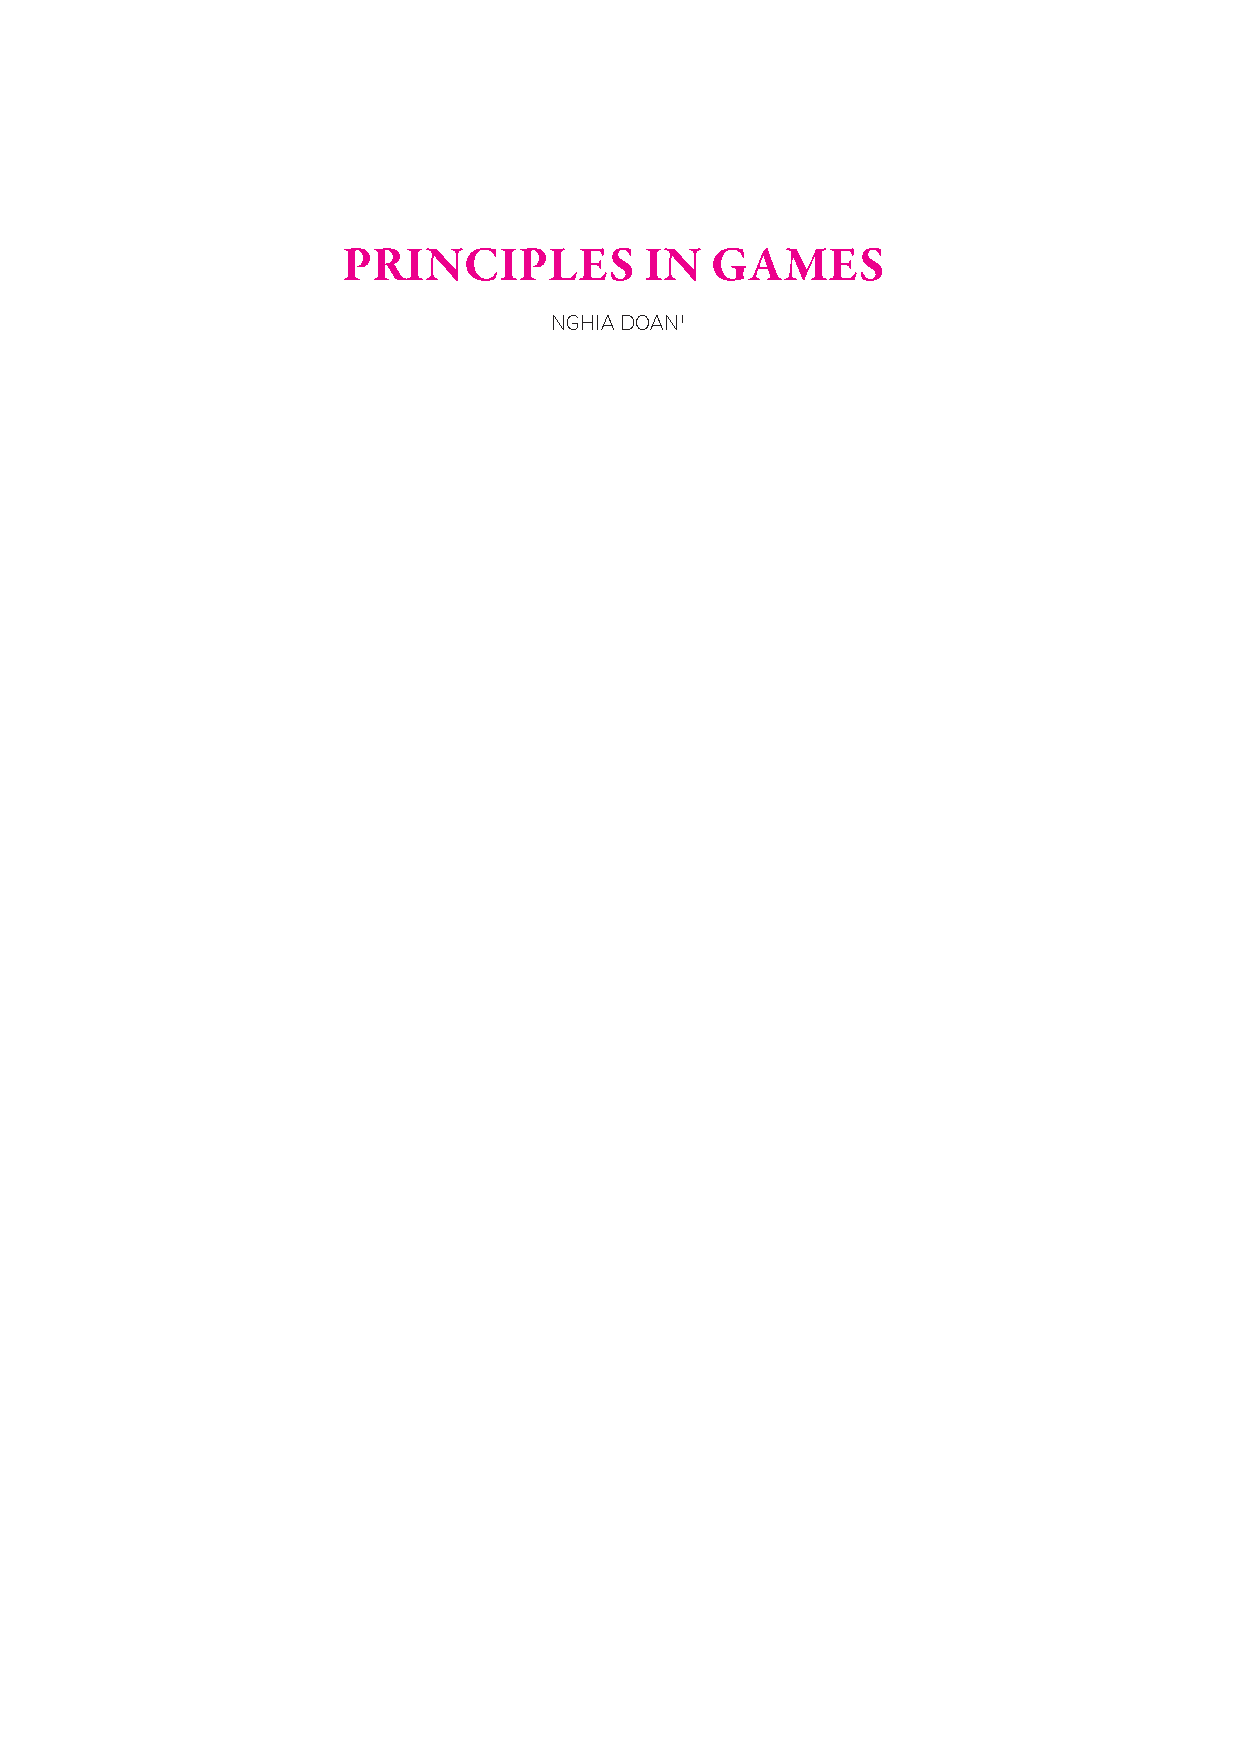
\includegraphics[scale=1]{../tieude6.pdf}}} 
%\centering
%\endgroup
%\graphicspath{{../toancuabi/pic/}}
%\vspace*{33pt}
%
%\begin{multicols}{2}
%	In this article, we discuss a few games and principles associated with solutions to the problems posed by the games.
%	\vskip 0.2cm
%	\PIbox{{\color{toancuabi}\textbf{Example} (Pigeons share a hole)\textbf{.}}
%		Each square of a $3 \times 3$ board is filled with one of the numbers $-1, 0, +1$. See the figure below for an example.
%		Viet calculates the sums of the rows, columns, and two main diagonals. He found that there are at least two equal sums.
%		For example, in the example below, both the sums of the second and third rows are $0$.
%		Is it always true that there are at least two equal sums?}
%	\vskip 0.1cm
%	\begin{figure}[H]
%		\vspace*{-5pt}
%		\centering
%		\captionsetup{labelformat= empty, justification=centering}
%		\begin{tikzpicture}[scale=0.78]
%			\draw (0,0) grid (3,3);
%			\draw (0.5,0.5) node {$-1$};
%			\draw (1.5,0.5) node {$+1$};
%			\draw (2.5,0.5) node {$0$};
%			\draw (0.5,1.5) node {$0$};
%			\draw (1.5,1.5) node {$-1$};
%			\draw (2.5,1.5) node {$+1$};
%			\draw (0.5,2.5) node {$-1$};
%			\draw (1.5,2.5) node {$+1$};
%			\draw (2.5,2.5) node {$+1$};
%		\end{tikzpicture}
%		\vspace*{-10pt}
%	\end{figure}
%	\textit{Solution.}
%	The answer is yes. The largest possible sum is $3$ and the smallest is $-3.$
%	So there are0 $7$ possible values $-3,-2,\ldots,2,3$ for $8$ sums, so two of them should be the same and therefore equal.
%	\vskip 0.1cm	
%	In above we applied the \textit{Pigeonhole principle: if $n+1$ or more pigeons are placed in $n$ holes, then one hole must contain two or more pigeons.} 
%	\vskip 0.2cm
%	\PIbox{{\color{toancuabi}\textbf{Example} (Nothing ever changes)\textbf{.}}
%	Each square of the  board contains a $+$ or $-$ signs, see the board the left,
%	which contains a single $-$ at the square intersection of the first row and second column.}
%	\vskip 0.1cm
%	\vspace*{0.1pt}
%	\vspace*{-8pt}
%	\PIbox{
%	At each step, you can change all the signs in a row, a column, or a diagonal to their opposite ones, i.e. $+$ to $-$, and $-$  to $+$.
%	An example of how a column is changed shown as below in the board on the right.}
%	\begin{center}
%		\begin{tikzpicture}[scale=0.78]
%			\draw [fill=cackithi!50] (1,0) rectangle (2,4);
%			\draw [fill=cackithi!50] (6,0) rectangle (7,4);
%			\draw (0,0) grid (4,4);
%			\draw (0.5,0.5) node {$+$};
%			\draw (1.5,0.5) node {$+$};
%			\draw (2.5,0.5) node {$+$};
%			\draw (3.5,0.5) node {$+$};
%			\draw (0.5,1.5) node {$+$};
%			\draw (1.5,1.5) node {$+$};
%			\draw (2.5,1.5) node {$+$};
%			\draw (3.5,1.5) node {$+$};
%			\draw (0.5,2.5) node {$+$};
%			\draw (1.5,2.5) node {$+$};
%			\draw (2.5,2.5) node {$+$};
%			\draw (3.5,2.5) node {$+$};
%			\draw (0.5,3.5) node {$+$};
%			\draw (1.5,3.5) node {$-$};
%			\draw (2.5,3.5) node {$+$};
%			\draw (3.5,3.5) node {$+$};
%			\draw (5,0) grid (9,4);
%			\draw (5.5,0.5) node {$+$};
%			\draw (6.5,0.5) node {$-$};
%			\draw (7.5,0.5) node {$+$};
%			\draw (8.5,0.5) node {$+$};
%			\draw (5.5,1.5) node {$+$};
%			\draw (6.5,1.5) node {$-$};
%			\draw (7.5,1.5) node {$+$};
%			\draw (8.5,1.5) node {$+$};
%			\draw (5.5,2.5) node {$+$};
%			\draw (6.5,2.5) node {$-$};
%			\draw (7.5,2.5) node {$+$};
%			\draw (8.5,2.5) node {$+$};
%			\draw (5.5,3.5) node {$+$};
%			\draw (6.5,3.5) node {$+$};
%			\draw (7.5,3.5) node {$+$};
%			\draw (8.5,3.5) node {$+$};
%		\end{tikzpicture}
%	\end{center}
%	\textit{Solution.}
%	Take a look at the squares colored \textcolor{red!50}{red}.
%	\begin{center}
%		\begin{tikzpicture}[scale=0.78]
%			\draw [fill=cackithi!50] (1,0) rectangle (2,4);
%			\draw [fill=cackithi!50] (6,0) rectangle (7,4);
%			\draw [fill=red!50] (0,1) rectangle (1,3);
%			\draw [fill=red!50] (1,3) rectangle (3,4);
%			\draw [fill=red!50] (3,3) rectangle (4,1);
%			\draw [fill=red!50] (3,1) rectangle (1,0);
%			\draw (0,0) grid (4,4);
%			\draw (0.5,0.5) node {$+1$};
%			\draw (1.5,0.5) node {$+1$};
%			\draw (2.5,0.5) node {$+1$};
%			\draw (3.5,0.5) node {$+1$};
%			\draw (0.5,1.5) node {$+1$};
%			\draw (1.5,1.5) node {$+1$};
%			\draw (2.5,1.5) node {$+1$};
%			\draw (3.5,1.5) node {$+1$};
%			\draw (0.5,2.5) node {$+1$};
%			\draw (1.5,2.5) node {$+1$};
%			\draw (2.5,2.5) node {$+1$};
%			\draw (3.5,2.5) node {$+1$};
%			\draw (0.5,3.5) node {$+1$};
%			\draw (1.5,3.5) node {$-1$};
%			\draw (2.5,3.5) node {$+1$};
%			\draw (3.5,3.5) node {$+1$};
%			\draw (5,0) grid (9,4);
%			\draw (5.5,0.5) node {$+1$};
%			\draw (6.5,0.5) node {$-1$};
%			\draw (7.5,0.5) node {$+1$};
%			\draw (8.5,0.5) node {$+1$};
%			\draw (5.5,1.5) node {$+1$};
%			\draw (6.5,1.5) node {$-1$};
%			\draw (7.5,1.5) node {$+1$};
%			\draw (8.5,1.5) node {$+1$};
%			\draw (5.5,2.5) node {$+1$};
%			\draw (6.5,2.5) node {$-1$};
%			\draw (7.5,2.5) node {$+1$};
%			\draw (8.5,2.5) node {$+1$};
%			\draw (5.5,3.5) node {$+1$};
%			\draw (6.5,3.5) node {$+1$};
%			\draw (7.5,3.5) node {$+$};
%			\draw (8.5,3.5) node {$+1$};
%		\end{tikzpicture}
%	\end{center}	
%	If we replace the $+$ sign by $+1$ and the $-$ sign by $-1$, then at the beginning the product of all numbers in these red square is $-1.$ 
%	Easy to see that each operation to change all the signs in a row, a column or a diagonal shall change exactly two red squares.
%	Whatever the numbers in the two red squares, the product of their negates remain same.
%	Since the product of the red squares at the beginning is $-1,$ so it cannot be changed at all.
%	\vskip 0.1cm
%	In above we applied the \textit{Invariant Principle: In mathematics, an invariant is a property of a mathematical object
%	(or a class of mathematical objects) which remains unchanged after operations or transformations of a certain type are applied to the objects.} 
%	\vskip 0.2cm
%	\PIbox{{\color{toancuabi}\textbf{Example} (Integers are well--ordered)\textbf{.}}
%	On a stormy night, ten students from the \textit{Math, Chess, and Coding Club in Ottawa} went to a party.
%	They left their shoes in the foyer in order to keep the carpet clean. After the dinner, there was a power outage.
%	So the students, leaving one by one, put on, at random, any pair of shoes big enough for their feet (each pair of shoes stay together).
%	Any student who couldn't find a pair of shoes big enough spent the night at the place of the party.
%	\vskip 0.1cm	
%	What is the largest number of students who might have had to spend the night? Show an example for this number.
%	\textit{Note that no two students wear the same size shoes.}}
%	\vskip 0.2cm
%	\textit{Solution.}
%	Easy to see that if the five students with smallest feet left first wearing all five largest pairs of shoes
%	then none of the remaining student can find a pair of shoes to leave.
%	Now let assume that there were $6$ students who would have to spent the night and there were $6$ pairs of shoes left,
%	then because $6 + 6 > 10,$ so there is a student with his pair of shoes is still at the place of the party. This is not possible!
%	\vskip 0.1cm
%	In above we applied the \textit{Well--Ordering Principle: the positive integers are well--ordered.
%	An ordered set is said to be well--ordered if each and every nonempty subset has a smallest or least element.} 
%	\vskip 0.2cm
%	\PIbox{{\color{toancuabi}\textbf{Example} (Invariant to reach end--state with desired outcomes)\textbf{.}}
%	In a darkroom there are two tables. The first one is empty and the second one is cover by a layer of nickels
%	(one nickel thick, so no coin is on top of another), in which $31$ coins are tails up and the rest are heads up.}
%	\vskip 0.1cm
%	\PIbox{
%	Minh enters the room with the task of transferring some coins from the second table to the first table
%	(he wears gloves, so he cannot feel the faces of the coins). He can flip over any number of coins when transferring them.
%	\vskip 0.1cm
%	Is that possible when he leaves the room the number of nickels that are tails up is the same on both tables?}
%	\vskip 0.2cm
%	\textit{Solution.}
%	If Minh turns a coin on the second table during transfer to the first one,
%	then the number of coins \textit{tails--up} on the second table will be reduce by one if it was a \textit{tails--p} coin,
%	or the number of coins \textit{tails--up} on the first table is increased by one if it was a \textit{heads--up} coin.
%	In any case, the difference between the \textit{tails--up} coins on the second and first tables will be reduced by one
%	(this is an \textit{invariant}.) Hence, after $31$ moves, they will be the same.
%	\vskip 0.1cm
%	In above we again applied the \textit{Invariant Principle} with a twist.
%	Note that in every turn the difference between the \textit{tails--up} coins on the second and first tables will be reduced by one,
%	since at the beginning, in other words, at the \textit{start state} this difference is $31,$
%	thus after $31$ turns the game reaches the \textit{end--state} where the difference is $0.$
%	\vskip 0.2cm
%	\PIbox{{\color{toancuabi}\textbf{Example} (Winning positions)\textbf{.}}
%	Berry and Cherry take alternate turns in playing a two--player game removing marbles from a pile as follows:
%	\vskip 0.1cm
%	$\bullet$ Berry always goes first.
%	\vskip 0.1cm
%	$\bullet$ The player whose turn it is, must remove exactly $2$, $4$, or $5$ marbles from the pile.
%	\vskip 0.1cm
%	$\bullet$ The player who at some point is unable to make a move (cannot remove $2$, $4$, or $5$ marbles from the pile) loses the game.
%	\vskip 0.1cm
%	They play $14$ games with $\{8, 9, \ldots, 21\}$ as the initial number of marbles in the pile.
%	What games does Cherry win, regardless of what Berry does?}
%	\vskip 0.2cm
%	\textit{Solution.}
%	The positive integers from $0$ to $21$ can be divided into 7 groups of numbers based on their remainders when divided by $7$,
%	\begin{align*}
%		&G_0=\{0,7,14,21\}, &&G_1=\{1,8,15\},\\
%		& G_2=\{2,9,16\}, &&G_3=\{3,10,17\},\\
%		& G_4=\{4,11,18\},&&G_5=\{5,12,19\},\\
%		& G_6=\{6,13,20\}
%	\end{align*}
%	It is easy to verify that,
%	\vskip 0.2cm
%	\PIbox{\textbf{\color{toancuabi}Claim.}
%		If $n$ is a number in $G_0$ and $G_1$ then $n-2$, $n-4$, and $n-5$ are in $G_2,G_3,G_4,G_5,$ or $G_6$.}
%	\vskip 0.2cm
%	Now, by the rules of the game, it is obvious that $\{0, 1\}$ are \textit{losing} positions and $\{2,4,5\}$ are \textit{winning} positions.
%	Furthermore, because $3-2=6-5=1$, so $\{3,6\}$ are also \textit{winning} positions, too.
%	\vskip 0.1cm
%	Therefore $G_0$ and $G_1$ contain all \textit{losing} positions, while $G_2,G_3,G_4,G_5,$ and $G_6$ containing all \textit{winning} positions.
%	A player, who is in a \textit{winning} position, can always force the game into a \textit{losing} position.
%	Thus, Cherry will win the game if the game starts with a \textit{losing} position.
%	Thus, the games that Cherry wins are $\{8,14,15,21\}$.
%\end{multicols}
